\documentclass[border=2pt]{standalone}
\usepackage{tikz}
\usetikzlibrary{arrows.meta,shapes.geometric,bending}
\begin{document}
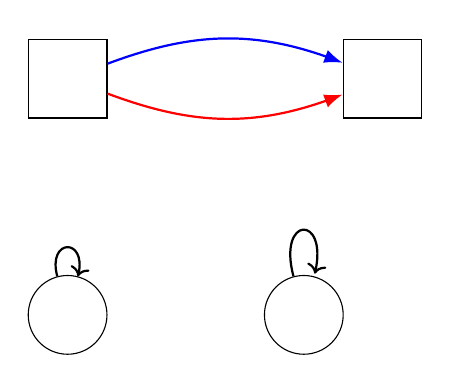
\begin{tikzpicture}
  \node[draw,minimum size=1cm,inner sep=0pt] (a) at (0,0) {};
  \node[draw,minimum size=1cm,inner sep=0pt] (b) at (4,0) {};
  \draw[-{Latex},thick,blue] (a) to[out=20.75,in=158.5] (b);
  \draw[-{Latex},thick,red] (a) to[out=-20.75,in=-158.5] (b);
  \node[circle,draw,minimum size=1cm,inner sep=0pt] (c) at (0,-3) {};
  \node[circle,draw,minimum size=1cm,inner sep=0pt] (d) at (3,-3) {};
  \path[->,thick] (c) edge[loop above,looseness=5] (c)
    (d) edge[loop above] (d);
\end{tikzpicture}
\end{document}
